\section{Ilham Muhammad Ariq (1174087)}
\subsection{Buku}
Rp.0 (Belum Lunas)
\subsection{Data Geospasial}
\begin{itemize}
	\item Pengertian Data Geospasial
	\par Geospasial terdiri dari dua kata, yaitu geo dan spasial, Geo berarti bumi sedangkan Spasial berarti ruang. UU No 4 tahun 2011 tentang geospasial menyebutkan, spasial adalah aspek keruangan dari suatu objek, atau yang mencakup lokasi,letak, dan posisinya. Data Geospasial dipecah menjadi dua, yaitu yang pertama;Data grafis atau geometri.Data ini terdiri dari tiga elemen: titik, garis, dan luasan. Data ini berbentuk vektor maupun raster. Kedua data tersebut adalah data atribut atau data tematik. Berikut penjelasan kedua data tersebut.
	
	\begin{enumerate}
	\item Data Vector
	\par Dalam bentuk data vector bagian objek dibumi ditampilkan sebagai kumpulan titik , garis dan polygon dimana sekumpulan tiitik yang saling terhubung akan membentuk garis dan garis yang saling terhubung antara titik awal dan titik akhir dengan nilai koordinat ynag sama akan membentuk polygon

	\begin{figure}[H]
	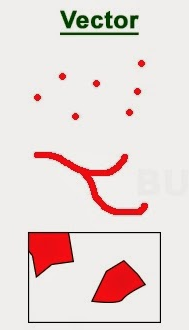
\includegraphics[width=4cm]{figures/Tugas1/1174087/vektor.png}
	\centering
	\caption{Data Vektor}
	\end{figure}
	
Data Vektor dibagi menjadi 2 yaitu :
	\begin{enumerate}
	\item Culture
	\par Culture memaparkan atau menampilkan data geospasial yang disertai dengan nama atribut atau memberikan 	keterangan atas nama dari objek di bumi. Contohnya nama dari suatu Negara, indicator batas air(keterangan kedalaman air laut), nama provinsi, daerah, wilayah dsb.
	
	\begin{figure}[H]
	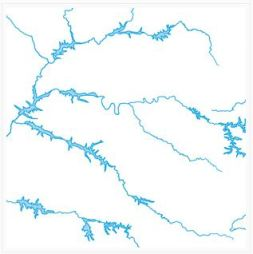
\includegraphics[width=4cm]{figures/Tugas1/1174087/lp.jpg}
	\centering
	\caption{Culture}
	\end{figure}
	
	\item Physical
	\par Physical memaparkan atau menampilkan data geospasial mengenai bentuk fisiknya atau gambaran tentang objek-objek alam yang ada dibumi. Contohnya gambaran laut, garis pantai, terumbu karang, danau dsb.
	
	\begin{figure}[H]
	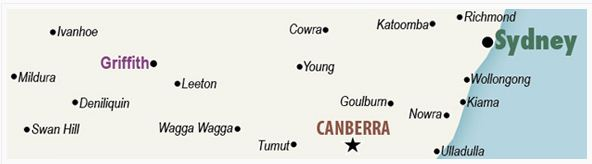
\includegraphics[width=4cm]{figures/Tugas1/1174087/pc.jpg}
	\centering
	\caption{Physycal}
	\end{figure}
	\end{enumerate}
	
	\item Data Raster
	\par Data raster menampilkan permukaan bumi seperti bentuk aslinya atau seperti dalam peta asli yang terlihat jelas dari setiap objek dengan keadaan alamnya. Data raster dibentuk atau menampilkan objek berupa elemen matriks atau grid , data raster digunakan untuk merepresentasikan objek dari data geospasial mengenai batas-batas yang berubah, ketinggian tanah dsb.

	\begin{figure}[H]
	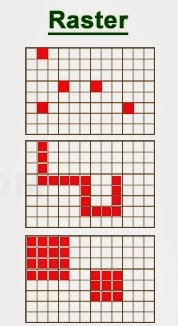
\includegraphics[width=4cm]{figures/Tugas1/1174087/raster.png}
	\centering
	\caption{Data Raster}
	\end{figure}
	\end{enumerate}
	
Dan adapaun software yang digunakan untuk mengolah data spasial atau membuat map kustom contohnya dapat menggunakan software QGIS dimana data yang akan diolah bisa didapatkan di web Natural Earth , ada data spasial berupa vector yang dibuat oleh ESRI (Environmental System Research Institute, Inc) dengan format data shapefile dan untuk data raster ada dengan format TIFF dengan TFW world file.
	
\end{itemize}

\subsection{Link}
\verb|https://youtu.be/iC4c71hMc_k|

\subsection{Plagiarism}
\begin{figure}[H]
	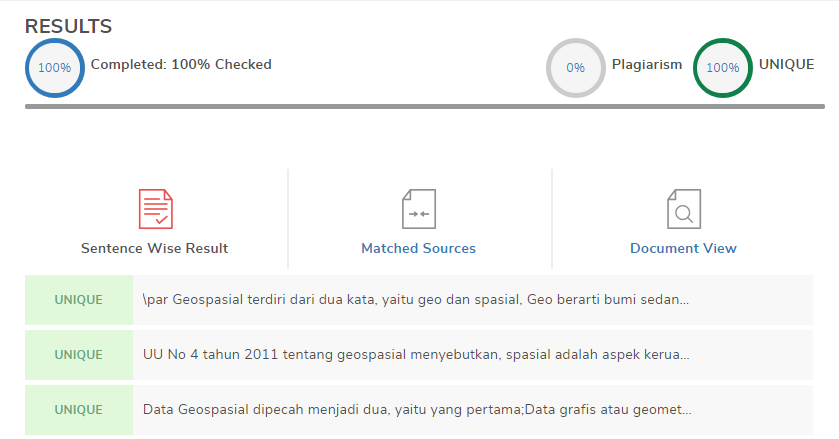
\includegraphics[width=4cm]{figures/Tugas1/1174087/plagiarism.png}
	\centering
	\caption{Plagiarism}
	\end{figure}